\documentclass[a4paper]{article}

\usepackage{caption}
\usepackage{listings}
\usepackage{fancyhdr}
\usepackage[top=3cm,bottom=3cm,left=3cm,right=3cm]{geometry}
\usepackage{color}
\usepackage{amsmath}
\usepackage{graphicx}
\usepackage{tabulary}

\definecolor{dkgreen}{rgb}{0,0.6,0}
\definecolor{gray}{rgb}{0.5,0.5,0.5}
\definecolor{mauve}{rgb}{0.58,0,0.82}

\lstset{frame=tb,
  language=Octave,
  aboveskip=3mm,
  belowskip=3mm,
  showstringspaces=false,
  columns=flexible,
  basicstyle={\small\ttfamily},
  numbers=none,
  numberstyle=\tiny\color{gray},
  keywordstyle=\color{blue},
  commentstyle=\color{dkgreen},
  stringstyle=\color{mauve},
  breaklines=true,
  breakatwhitespace=true,
  tabsize=3
}

\newcommand{\HRule}{\rule{\linewidth}{0.5mm}}
\pagestyle{fancy}
\lfoot{\small \color{gray}Tom Peerdeman - 10266186}
\cfoot{\thepage}
\rfoot{\small \color{gray}Ren\'e Aparicio Sa\'ez - 10214054}
\lhead{\small \color{gray}Autonome Mobiele Robots}

\begin{document}
\begin{titlepage}
\begin{center}
\textsc{\Large Autonome Mobiele Robots}\\[0.5cm]
\HRule \\[0,4cm]
\textsc{\huge \bfseries NXT - Particle filter based simultaneous localization and mapping}
\HRule \\[8cm]
\begin{minipage}{0.4\textwidth}
\begin{flushleft}\large
\emph{Auteurs: Tom Peerdeman \& Ren\'e Aparicio Saez}\\
\end{flushleft}
\end{minipage}
\begin{minipage}{0.4\textwidth}
\begin{flushright}\large
\emph{Datum: \today\\\hspace{1cm}}\\
\end{flushright}
\end{minipage}
\end{center}
\end{titlepage}

\tableofcontents
\newpage

\section{Materiaal}
Om de experimenten uit dit rapport te kunnen uitvoeren zijn de volgende materialen gebruikt:\\
- PC/Laptop met Matlab\\
- Boek: Autonomous Mobile Robots 2th Edition - Roland Siegwart et al.\\
- NXT-Robot\\
- Logitech Webcam\\
- Gloeilamp\\
- Zwarte tape

\section{Introduction}
Een autonome mobiele robots moet een kaart kunnen opbouwen van zijn omgeving. Aan de hand van zijn eigen gemaakte kaart zou hij met behulp van bekende kaarten kunnen bepalen waar hij zich in de wereld bevindt. Een veel gebruikte methode om een kaart al rijdend op te bouwen is SLAM (Simultaneous Localization And Mapping). Er kan dan met een bepaalde zekerheid bepaald worden waar de robot zich momenteel bevindt. Het is de bedoeling dat de robot in een gebied rond kan rijden en hierbij een goede kaart kan maken. Zo moet hij bijvoorbeeld na het rijden van een rondje weer hetzelfde deel van de kaart zien (mits er niks veranderd is aan de omgeving).

\section{Feature detection}
De gebruikte versie van SLAM, fastSLAM, maakt gebruik van ruwe odometrie data en features welke gedetecteerd worden door de laserscan.
Als feature zal gebruik gemaakt worden van hoeken van lijnen. Om de corners te kunnen vinden zullen eerst de lijnen gevonden moeten worden uit de ruwe punten data die de laserscan aanlevert. Om deze lijnen te kunnen detecteren wordt gebruik gemaakt van het split \& merge algoritme. Het split en merge algoritme is in stappen uitgelegd in listing \ref{lst:splitmerge}.

\begin{lstlisting}[caption= Split \& merge algorithm, label=lst:splitmerge, numbers=left]
Initially: set s1 consists of all N points. Insert s1 to the list L. Set index i=1
Fit a line to the next set si in L
Detect the point P with the maximum distance D to the line
if D is less than a threshold then continue to step 2
else split si at P into si1 and si2, replace si , in L, by si1 and si2. Continue to step 2
When all sets (segments) in L have been checked, merge collinear segments.
\end{lstlisting}

\noindent Het fitten van een lijn wordt hierbij gedaan door het zoeken naar een lijn zodanig dat de som van de afstanden van de punten tot de lijn minimaal is. De lijn wordt hierbij uitgedrukt in polaire co\"ordinaten $r$ en $\alpha$ (zie figuur \ref{fig:linefit}).

\begin{figure}[h]
	\centering
	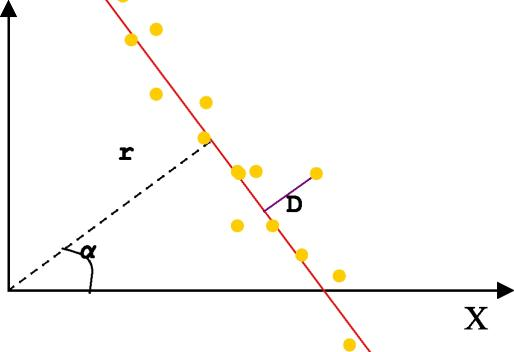
\includegraphics[width=0.7\textwidth]{img/stolenline.png}
	\caption{Fitten van de lijn door de som van D te minimaliseren}
	\label{fig:linefit}
\end{figure}


\section{Deel 1, Gegeven data}
\subsection{Formules}
\subsection{Parameters bepalen}
\section{Deel 2, Eigen data}
\subsection{Offline SLAM met behulp van een dataset}
\subsection{Odometrie bepalen}
\subsection{Resultaten}
\subsection{Discussie}
\subsection{Verbeteringen}


\end{document}
